\chapter{Spoken Dialogue Systems}
\label{chap:spoken_dialogue_systems}

\lettrine{T}{his} chapter gives an overview of the \aclp{sds} paradigm, including common architectures, different system types, and evaluation methods.
The concept of adaptive \aclp{sds}, which is a core idea in this work, is introduced as well, along with examples of adaptation on different levels.

\pagebreak

%\section{What is a spoken dialogue system?}
%\label{sec:what_is_a_sds}

\todo[inline]{here talk about what is a dialogue, a spoken dialogue, turn, when an interaction becomes a dialogue (is every interaction with a machine is a dialogue system?), etc. can really use the introductions given by Olga in the SDS seminar}

Nowadays, \acfp{sds} are used in various forms in our everyday life.
Giving users all the features of a responsive (sometimes personalized, see \cref{subsec:personal_assistants}) dialogue system with the advantage of using voice to communicate, leaving the hands free to perform any other action, such as driving.\\

In recent years, the market for commercial \acp{va} has rapidly grown.
For example, Microsoft Cortana had 133 million active users in 2016 \citep{Osborne2016why} and Echo Dot was Amazon's best-selling product between 2016 and 2018 \citep{Dickey2017echo}.
Furthermore, \SI{72}{\percent} of people who own a smart speaker say they often use their devices as part of their daily routine \citep{Kleinberg2018ways}.

\todo[inline]{give examples of commercial systems and places where SDSs are used}

\section{Types of spoken dialogue systems}
\label{sec:types_of_sdss}

\todo[inline]{short general introduction explaining the term ``computer-based'' agent as a overarching term for all of the other listed below.}

\begin{table}[tb]
	\centering
	\caption[Types of \aclp{sds}: Task-oriented vs.\ Chit-chats]{A comparison between task-oriented \acp{sds} and chatbots.}
	\label{tab:sds_types}
	\begin{tabulary}{\linewidth}{>{\bfseries}lCC}
		\toprule
							&   {\large \textbf{Task-oriented}}																	& {\large \textbf{Chit-chats}}													\\
		Goal				&	Helps the user achieve a specific, defined goal													& No specific goal, aims to converse as naturally and continuously as possible	\\
		Applications		&	\Aclp{pa}, \acl{cnc} systems, integrated voice-activated systems for cars, reservations, etc.	& Chatbos, social robots, conversational AI										\\
		Domain				&	Domain-specific, possibly multi-domain															& Aims to be domain-free (a.k.a.\ open domain)									\\
		Modeling			&	Statistical models and/or handcrafted rules 													& Typically sequence-to-sequence models with no-go filters						\\
		Evaluation			&	Task completion rate and completion time, number of turns (+ subjective criteria) 				& Chat length, relevant replies ratio, general user satisfaction				\\
	
		\bottomrule
	\end{tabulary}
\end{table}

\subsection{Personal assistants}
\label{subsec:personal_assistants}

\Acp{pa}\ldots

A big advantage of \acp{va} is their simple operation.
Using nothing but speech commands, users can perform tasks like playing music, searching the web, shopping online, etc.
In the future, we are likely to witness an ever-growing presence of devices with spoken interaction capabilities, like speech-activated cars, hands-free medical assistants, and intelligent tutoring systems.
This will increase the demands on voice-activated devices even more, as they will need to support more functionalities in a way that is comfortable and intuitive for the users.
Additionally, it can be expected that such devices will be used not only by individuals, but also in more social contexts, i.e., where multiple humans are involved.


Besides making the operation of such voice-activated systems simple and user-friendly, \acp{pa} also aim to let users interact with them in a familiar, natural manner.
One property of natural interactions is the tendency to accommodate to the specific situation and interlocutors to make the interactions more fluent and efficient \citep{Giles1991CAT,Gallois2015CAT}.
Linguistic accommodation is one aspect of this phenomenon, and it is found in various \ac{hhi} experiments \citep[e.g.,][]{Pardo2017phonetic,Schweitzer2017social}.

\subsection{Intelligent speakers}
\label{subsec:intelligent_speakers}

\Acp{pa} are sometimes integrated into a loudspeaker that can be placed in a central spot at home or in an office\ldots

\subsection{Chatbots and social robots}
\label{subsec:chatbots}

Chatbots (sometimes also called \emph{chatterbots} or \emph{chitchat bots}) are a\ldots

\todo{write a bit about history of chatbots (start with ALICE)}

Chatbots have been used in various domains such as education \citep{Benotti2014engaging, Kerly2007bringing}, culture heritage \citep{Pilato2005expert}, healthcare \citep{Kowatsch2017text}, software development \citep{Lebeuf2017software}, and others \citep{Shawar2007chatbots}.

\subsection{Embodied agents}
\label{subsec:embodied_agents}

\subsection{Virtual agents and virtual humans}
\label{subsec:virtual_agents}

Also known as \textit{avatars}, these...

\section{Architecture of spoken dialogue systems}
\label{sec:architecture_sds}

\todo[inline]{explain that this is a generic, symmetric architecture. there are sometimes some extensions or sub-components to some of the modules}
\todo[inline]{explain that each of the components is a research area by its own}

\begin{figure}[t]
	\centering
	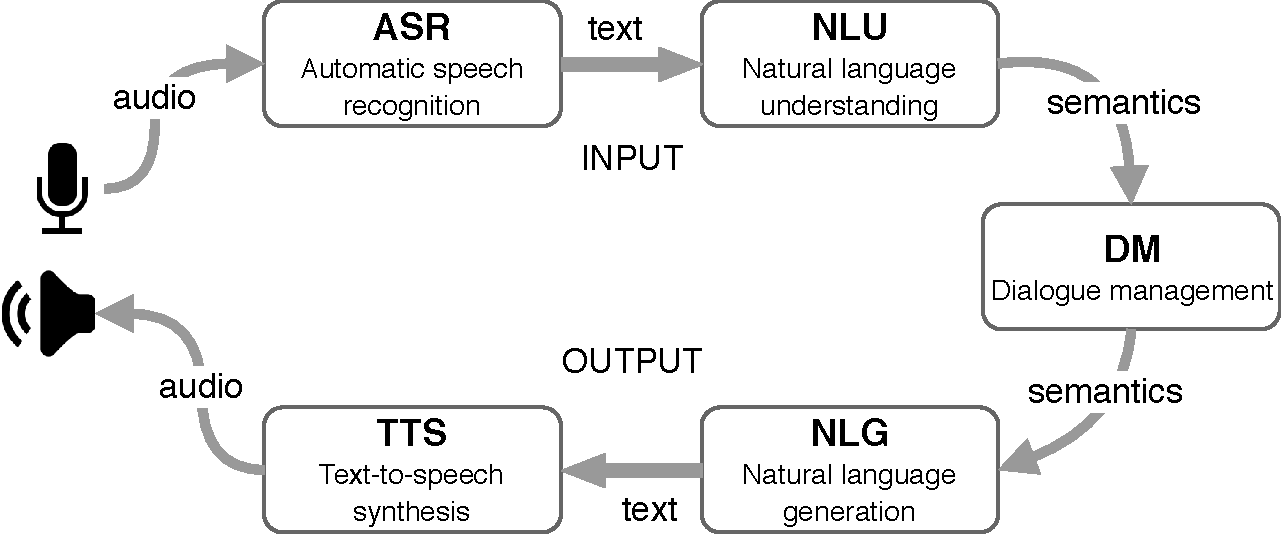
\includegraphics[width=\linewidth]{sds_architecture}
	\caption[Architecture of a spoken dialogue system] {
		A typical architecture of a spoken dialogue system.
		The interaction lifecycle is symmetric, and for each analysis input step there is a corresponding generation output step.
		The exchange usually starts with a user spoken utterance and ends with the system's spoken response.
	}
	\label{fig:sds_architecture}
\end{figure}

Each of a the components shown in \cref{fig:sds_architecture} is a whole research area by itself.
Brief overviews is given here, along with some systems and implementation that can be used for each of these \ac{nlp} task:

\subsection{Automatic speech recognition}
\label{subsec:automatic_speech_recognition}

\subsubsection{Tools}
\label{subsubsec:tools_asr}

\subsection{Natural language understanding}
\label{subsec:natural_language_understanding}

\todo[inline]{be sure to mention the term \enquote{intention}}

\subsubsection{Tools}
\label{subsubsec:tools_nlu}

\subsection{\Acl{dm}}
\label{subsec:dialogue_management}

\todo[inline]{short-mid-length intro to this. about purpose, importance, "core of the SDS", etc.}
\ldots is typically divided into \emph{Belief Tracker} and \emph{Policy}.
\todo[inline]{Now explain about each of them. former is about past turns and anticipating the user's intent, latter is about future responses and what response best matches the user's needs/expectations. mention the use of Reinforcemnet Learning, since it is used when feedback from user is used to improve a system. there are probably papers where this is used.}
\todo[inline]{also explain that this is the part that is connected to external resources, if necessary}

Another component of the \ac{dm} is the \emph{domain}\ldots
Some external knowledge base can be connected as well\ldots
The domain determines what the system can talk about and react to, and to what extent.
\todo[inline]{examples of (simple) domain}
\todo[inline]{combining domains and extending domains, e.g. using crowd sourcing or machine learning}
\todo[inline]{breadth vs.\ depth of domain in SDS (variety vs.\ complexity). replicate the graph Milica showed in her talk (x-axis is breadth and y-axis depth, with some examples along combinations of the axes.)}
\subsubsection{Tools}
\label{subsubsec:tools_dm}

\subsection{Natural language generation}
\label{subsec:natural_language_generation}

\subsubsection{Tools}
\label{subsubsec:tools_nlg}

\subsection{Text-to-speech synthesis}
\label{subsec:text-to-speech_synthesis}

\subsubsection{Tools}
\label{subsubsec:tools_tts}

\section{Adaptive spoken dialogue systems}
\label{sec:adaptive_spoken_dialogue_systems}

\todo[inline]{taken as-is from the submitted version of SIGdial 2018 paper, add more based on existing adapting systems on different levels. need to expand, and add detailed parts about each of the things that can be adapted. get more names of implemented system (maybe even pictures), and mention algorithms etc.}

Various studies have investigated entrainment and priming in \acp{sds}, aiming to better understand \ac{hci} dynamics and improve task-completion performance.
\citet{Lopes2013automated, Lopes2011primes}, for example, focused on dynamic entrainment and adaptation on the lexical level.
Others, like \citet{Nenkova2008high}, concentrated on word frequency.
\citet{Parent2010lexical} examined changes in both lexical choices and word frequency using the \emph{Let's Go} \ac{sds} \citep{Raux2005letsgo}.
While these studies addressed the changes in experimental, scripted scenarios, the theoretical foundations for studying these changes in spontaneous dialogue exist as well \citep{Brennan1996lexical}.
\citet{Gasic2013policy, Levin2000stochastic} provide examples of online adaptation for dialogue policies and strategies.

It is important to note that while all of the studies mentioned above examine various aspects of dialogues, none of those are related to speech -- the primary modality used to interact with \acp{sds}.
Studying convergence in speech in an \ac{hci} context is made possible with more natural synthesis technology, which gives more fine-grained control over parameters of the system's spoken output.
\todo{need references here?}
Many systems that deal with adaptation of speech-related features focus on prosodic characteristics like intonation or speech rate.
\citet{Levitan2014acoustic} sheds light on acoustic-prosodic entrainment in both \ac{hhi} and \ac{hci} via the use of interactive avatars.
\citet{Bell2003prosodic} found that users' speech rate can be manipulated using a simulated \ac{sds}.
Similar results were found when intensity changes in children's interaction with synthesized \ac{tts} output were examined \citep{Coulston2002amplitude}.
A technical overview of the development of adaptive \acp{sds} is given by \citet{Levitan2016implementing}, where speech rate and intensity are manipulated and entrained by the system.

All of the above provide solid ground for further investigation of phonetic convergence in \ac{hci} using \acp{sds}.

\section{Evaluating spoken dialogue systems}
\label{sec:evaluation_of_sdss}

\ldots Therefore, evaluation of \acp{sds} depends on the purpose of the systems, which can be divided into two types, namely \textit{\aclp{tds}} and \textit{\aclp{ngs}}.

\subsection{Task-Driven Systems}
\label{subsec:taskdrivensystems}
[doesn't really evaluate the \ac{sds}, but it's ability to predict what task should be performed]
[typically part of a bigger system (which has a set of tasks it can perform (e.g. personal assistant))]

\subsection{Non-Goal Systems}
\label{nongoalsystems}

A \acf{ngs} is a \ac{sds} that does not necessarily aim to complete a specific task (unlike \acp{tds}).
Its purpose is, then, more general and there might not even be a defined purpose for it.
Chatbots (see \cref{subsec:chatbots}) are a good a example for a \ac{sds} that typically isn't used for accomplishing a practical task like getting information or operating a device.
Instead, they are used as a long-term social companion (be it at home or as part of a mobile device) and even merely for entertainment. \todo{references for both examples}
Since such systems don't help achieving a defined goal, it is not possible to evaluate their performance based on how well (or whether at all) this goal task was carried out.
There is a need therefore for another, more long-term and interaction-oriented method rather than a task-oriented method.
On the one hand, from the \ac{hci} point of view, the advantage of such methods is that they evaluate the dialogue capabilities of the system and not merely it's ability to map speech patterns or keywords to a set pre-defined actions.
On the other hand, however, the problem in such methods is that it is much harder to define metrics when the goal of the interaction is not completely defined.
There are two approaches to solve this issue:
The first is defining the 
